
\chapter{ELEKTROMAGNETISKA FÄLT}

\section{INLEDNING}
\index{elektromagnetiska fält (EMF)}
\index{EMF}
En amatörradiostation genererar signaler för att kommunicera trådlöst
med hela världen. Detta sker med signaler som kallas elektromagnetiska
fält (EMF). Runt alla sändande antenner bildas EMF av den energi som
skickas in i dem från sändaren, fälten kallas vanligen radiovågor.

Radiovågorna (EMF) är klassificerade som \emph{icke-joniserande strålning}.

Icke-joniserande elektromagnetisk strålning, vilket är samma sak som
elektromagnetiska fält (EMF), uppträder i många former. Som radiovågor,
mikrovågor, infraröd strålning, synligt ljus, ultraviolett strålning.
Det som skiljer är våglängden. Radiovågor har längst våglängd och
ultraviolett kortast.

\index{joniserande strålning}
\index{strålning!joniserande}
Joniserande strålning är så energirik att den kan rycka loss
elektroner från de atomer som den träffar och förvandla dem till
positivt laddade joner, jonisering. Exempel på joniserande
strålning är röntgenstrålning och strålning från radioaktiva ämnen.
Energin hos den joniserande strålningen kan vara så hög att den kan
tränga in i och påverka cellstrukturen i biologiskt material.

\index{icke-joniserande strålning}
\index{strålning!icke-joniserande}
Energin hos icke-joniserande strålning, som optisk strålning och
elektromagnetiska fält, är normalt inte lika energirik som de
joniserande och kan därför inte jonisera material utan orsakar enbart
uppvärmning av kroppens vävnad. I allmänhet har studier visat att de
nivåer av EMF som allmänheten utsätts för ligger långt under de värden
där kroppstemperaturen skulle öka.

En amatörradiostation genererar således enbart icke-joniserande
strålning vilken absolut inte får blandas ihop med vad som kallas
joniserande strålning. Det är därför mycket viktigt att förstå
skillnaden mellan dem.

\index{WHO}
\index{World Health Organizatio (WHO)}
\index{International Commission on Non-Ionizing Radiation Protection (ICNIRP)}
\index{ICNIRP}
Inom World Health Organization (WHO) finns ett program som kallas
’The International EMF Project’ och där samlas all vetenskaplig
information som finns om biologiska effekter av elektromagnetiska fält.
’International Commission on Non-Ionizing Radiation Protection’, (ICNIRP)
är en fristående organisation (erkänd av WHO) som bland annat använder denna
information för att utveckla riktlinjer för begränsning exponering för EMF.
Dessa riktlinjer används av många länder.

\index{Strålsäkerhetsmyndigheten (SSM)}
\index{SSM}
Strålsäkerhetsmyndigheten (SSM) är den myndighet som arbetar med
ovanstående frågor i Sverige har tagit fram allmänna råd som är
en tolkning av ett EU-direktiv som bygger på ICNIRP:s riktlinjer för
allmänhetens exponering för elektromagnetiska fält.

Eftersom grunden i amatörradioutövandet är att generera
elektromagnetiska fält för att kommunicera via radio så är kunskapen
om EMF viktig. Med de befogenheter radioamatörer har, måste de
allmänna råden för EMF följas och förståelsen för hur fält uppstår
och hur de kan begränsas är fundamental.

\section{FÄLT}
Antennens uppgift är att omvandla den ledningsbundna signalen i
matarkabel på ett så effektivt sätt som möjligt till en
elektromagnetisk våg som utbreder sig i luften.

Den elektromagnetiska vågen uppträder inte direkt vid antennen utan
uppstår i det som man kallar fjärrfältet. Detta sker genom växelverkan
mellan det elektriska och magnetiska fältet som antennen genererar.

\index{närfält}
\index{fjärrfält}
Teorierna som beskriver hur denna växelverkan fungerar är komplicerade
men det viktiga att förstå är att det finns en gräns mellan vad man
kallar fjärrfältet längre bort från antennen och närfältet nära
antennen. Av denna anledning måste man nära antenner mäta både det
elektriska- och det magnetiska fältet för att utvärdera maximal fältstyrka.
I fjärrfältet kan man på grund av växelverkan mellan dem
mäta antingen det ena eller det andra.

Beroende på den antenntyp som genererar fältet är det antingen ett
elektriskt eller magnetiskt fält som dominerar i närfältet.
Elektrisk fältdominans genereras av antenntyper som bygger på
spänningsskillnader (tex dipol) och magnetisk fältdominans av antenner
med strömflöde (tex. små loopar).

\index{elektriskt fält (E)}
\index{magnetiskt fält (H)}
Det elektriska fältet (E) anges i ”volt per meter” (V/m) och det
magnetiska fältet (H) i ”ampere per meter” (A/m).

I och med att fältet utbreder sig i luften åt alla håll samtidigt så
avtar styrkan i fältet. Detta beror på att effekten som genererar
fältstyrkan runt antennen täcker ett större och större klot ju
längre bort man kommer. Effekten per ytenhet minskar därmed på
längre avstånd från antennen.

Fältet avtar alltså i styrka på samma sätt som att jämföra ytan på två
klot med olika radier. Genom matematisk analys av dessa klots ytor med
olika radier kommer man fram till att om avståndet dubbleras halveras
fältstyrkan.

Det spelar ingen roll om antennen är helt rundstrålande eller
koncentrerar effekten i en riktning, fältet avtar på samma sätt i
alla fall.

Eftersom alla elektriska ledare kan betraktas som antenner kommer
dessa att kunna generera fält, oavsett om det är tänkt att det ska
vara en antenn eller inte. Detta är tydligt då både apparater och
ledningar kan leda högfrekvent ström och genom detta generera fält.
Man bör ha detta i åtanke vid installation av matarledning till
antennen för att undvika att ström flyter tillbaka till stationen på
utsidan av ledningen. Även de apparater man använder för att generera
de signaler man vill skicka ut kan ha dålig skärmning och leda
högfrekvent ström på utsidan.

Det finns alltså en risk att fältstyrkorna i närheten av sändare, och
framför allt slutsteg med tillhörande kablage, kan vara betydande.

\section{ALLMÄNNA RÅD}

\index{Strålsäkerhetsmyndigheten (SSM)}
\index{SSM}
Strålsäkerhetsmyndigheten (SSM) är den myndighet som är sammanhållande
för allmänhetens exponering för elektromagnetiska fält. Dess allmänna
råd, SSMFS 2008:18, anger vilka referensvärden som gäller i Sverige.

\index{ICNIRP}
Syftet med de allmänna råden är att skydda allmänheten från akuta
skadliga biologiska effekter vid exponering för elektromagnetiska fält.
De allmänna råden är en svensk anpassning av ett EU-direktiv som
grundar sig på ICNIRP’s riktlinjer.

\index{Specific Absorption Rate (SAR)}
\index{SAR}
Riktlinjerna baseras på hur kroppen värms upp av radiovågorna och
definieras som: hur stor effekt per kilogram kroppsvikt som absorberas
under en definierad tid. Den tekniska benämningen på detta värde är
’Specific Absorption Rate’ (SAR) och mäts i W/kg.
De grundläggande begränsningarna är, enligt internationella
rekommendationer, satta vid ungefär två procent av de nivåer vid
vilka akuta biologiska effekter är vetenskapligt säkerställda.

Då uppvärmningen av kroppsvävnad inte går snabbt räknar man med den
medeleffekt som under en viss tid orsakar uppvärmning. De allmänna
råden definierar SAR-värdet som medelvärdet under en sexminutersperiod.

Eftersom ett elektromagnetiskt fält inte går att mäta i enheten W/kg
innehåller de allmänna råden även en tabell på referensvärden
framräknade för att motsvara SAR-värdet. Referensvärdena utgörs av
storheter som är mätbara utanför människokroppen.

Referensvärdena är angivna i bland annat elektrisk- och
magnetisk-fältstyrka, vilka är mätbara storheter. De är också de
värden som en amatörradiostation inte bör överskrida i områden där
allmänheten kan vistas.

Vid frekvenser som är nära kroppens egen resonansfrekvens absorberas
effekten lättast och maximal uppvärmning uppstår. Hos vuxna ligger
den frekvensen på ungefär 35~MHz om personen är jordad och vid
ungefär 70~MHz om personen är isolerad från jord. Även de olika
kroppsdelarna kan vara resonanta. T.ex. är en vuxens huvud resonant
vid ca 400~MHz medan ett mindre barns huvud är resonant vid ca 700~MHz.

Kroppens storlek avgör alltså vid vilken frekvens den absorberar mest
effekt och vid frekvenser över och under resonansfrekvensen så minskar
uppvärmningen från fältet.

Referensvärdena tar hänsyn till detta faktum och det mest restriktiva
frekvensområdet ligger inom 10 till 400~MHz vilket är där effekten
absorberas lättast av kroppen.

\begin{figure*}[h]
\begin{center}
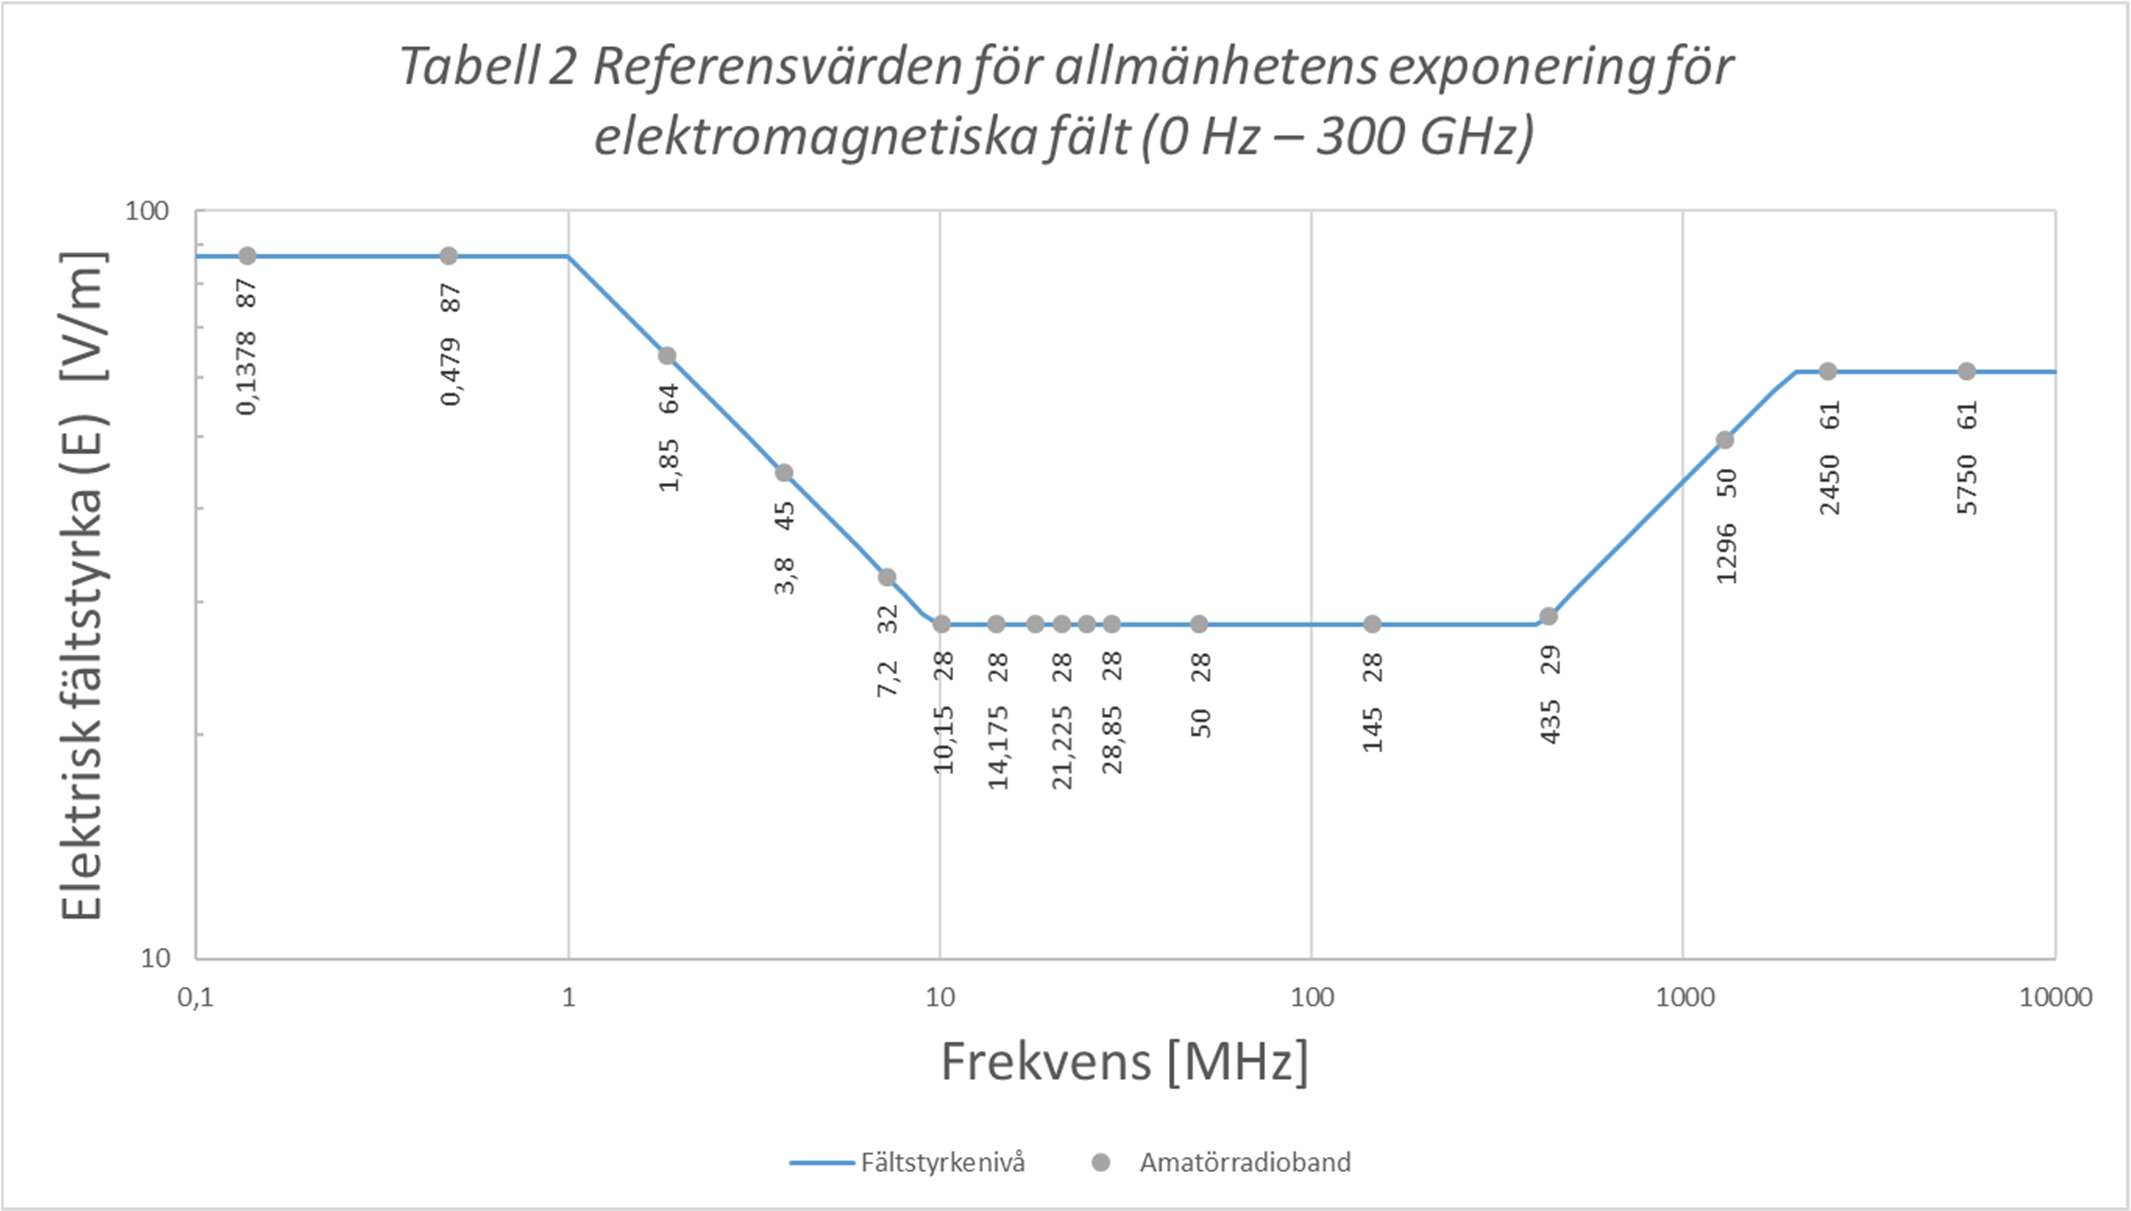
\includegraphics[width=14cm]{images/emfbild-000}
\caption{Referensvärden för allmänhetens exponering för elektromagnetiska fält (0~Hz -- 300~GHz)}
\label{fig:emf1}
\end{center}
\end{figure*}

Bild \ref{fig:emf1} illustrerar referensvärden för allmänhetens
exponering för elektriska fält (0~Hz -- 300~GHz), med amatörband
och fältstyrkenivå angivna, t.ex. 10,15~MHz har en högsta tillåtna
elektriskt fältstyrka på 28~V/m.

\begin{figure*}[h]
\begin{center}
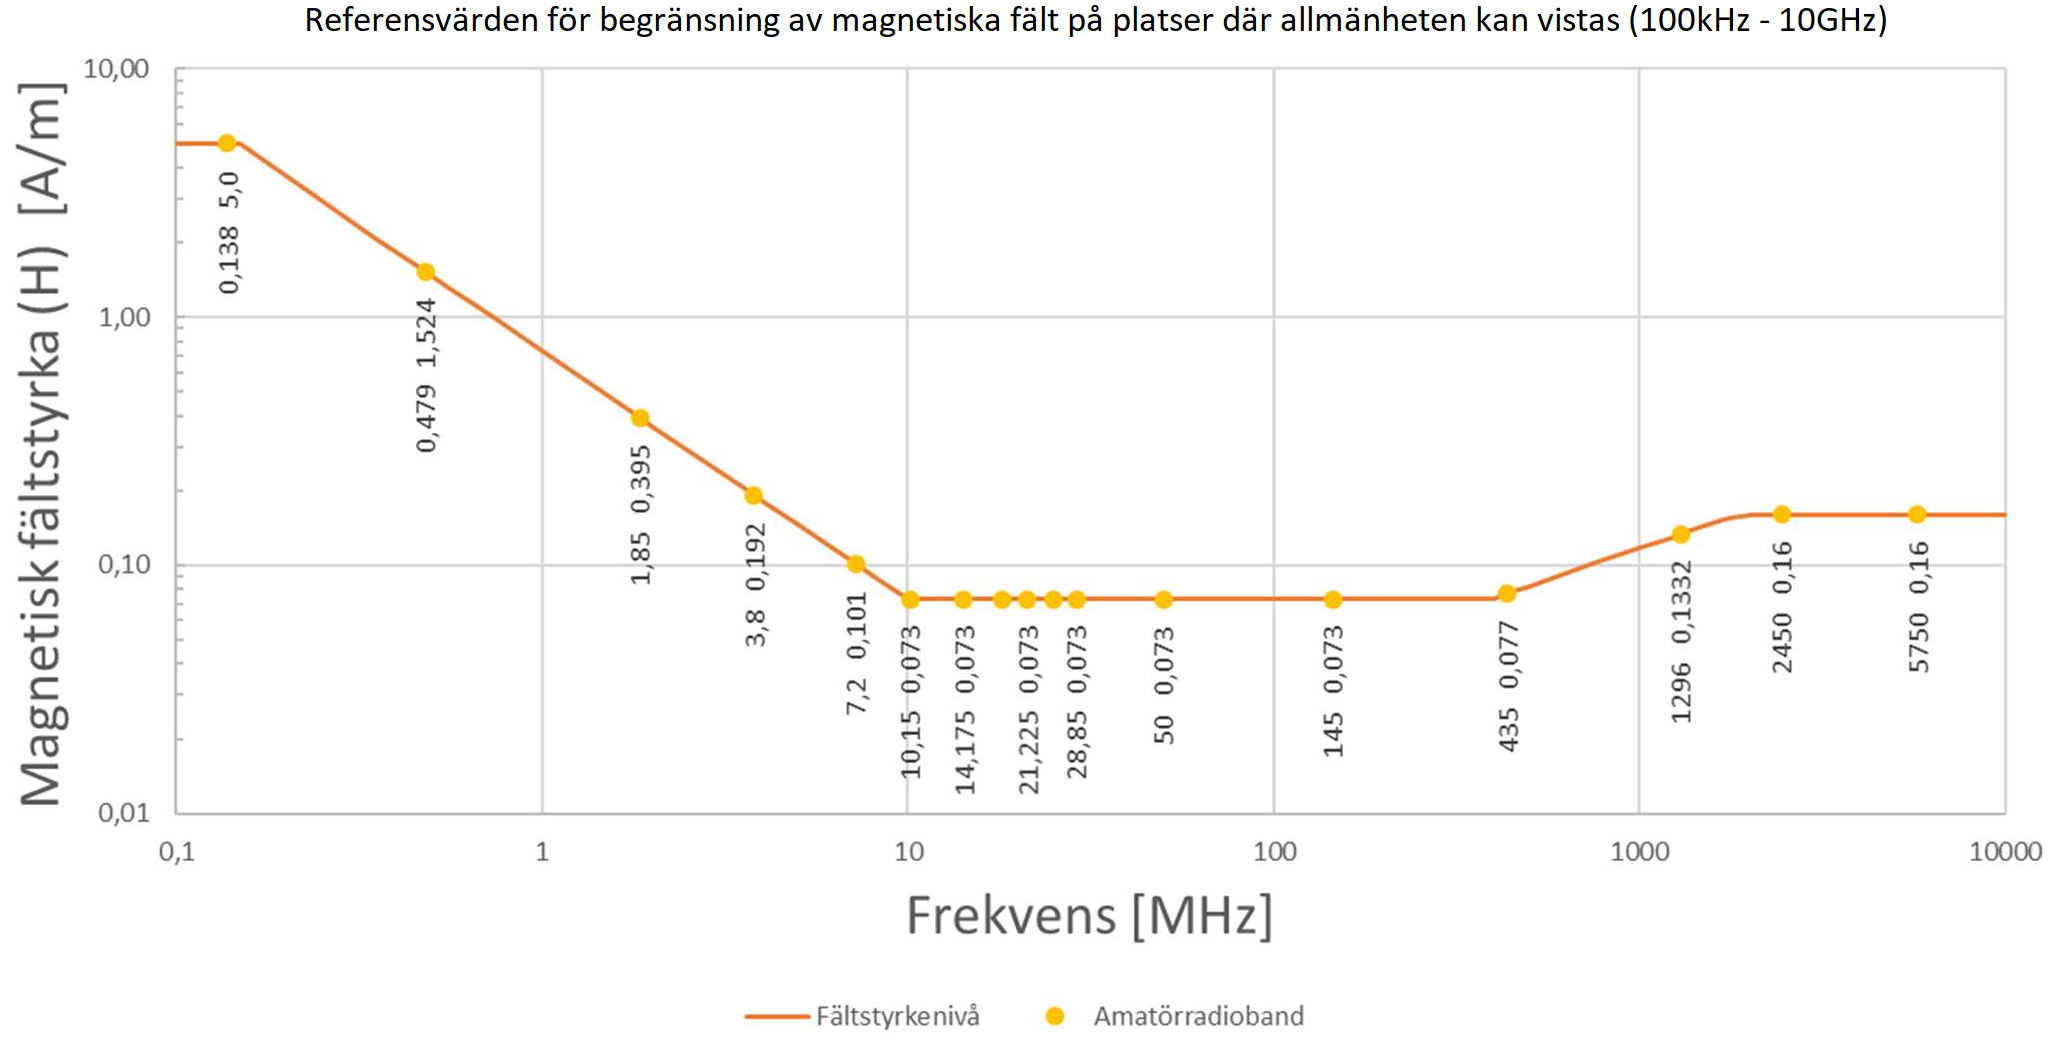
\includegraphics[width=14cm]{images/emfbild-001}
\caption{Referensvärden för allmänhetens exponering för elektromagnetiska fält (0~Hz -- 300~GHz)}
\label{fig:emf2}
\end{center}
\end{figure*}

Bild \ref{fig:emf2} illustrerar referensvärden för allmänhetens
exponering för magnetiskt fält (0~Hz -- 300~GHz), med amatörband
och fältstyrkenivå angivna, t.ex. 10,15~MHz har en högsta tillåtna
magnetisk fältstyrka på 73~mA/m.

\section{UTVÄRDERING AV EMF}

Hur är det då med den egna stationen, överensstämmer fältstyrkorna som
den kan generera med referensvärdena?

För att kunna utvärdera detta måste man känna till vilka parametrar
som är avgörande vid en beräkning av fältstyrkan. Mycket beror på
vilken antenn man använder och hur den är placerad.
Man måste även förstå egenskaperna signalen från sändaren har.

\subsection{Antennen}

Antennen tar emot signalen från sändaren via en matningskabel och
omvandlar denna signal till en elektromagnetisk våg. Hur denna
omvandling går till är komplicerat men kan enklast förklaras med
begreppet förstärkning eller antennvinst. Man måste alltså känna
till vilken förstärkning antennen har. Formeln som används för
uträkning av fältstyrkan förutsätter att man benämner antennens
förstärkning relativt en isotrop antenn (dBi) och inte en
dipolantenn (dBd), samt att man räknar med linjära värden (gånger)
och inte logaritmiska (dB).

\begin{tabular}{|l|ccccccccccc|}
\hline
dB     &  0  &  1  &  2  &  3  &  4  &  5  &  6  &  7  &  8  &  9  & \\ \hline
Gånger & 1,0 & 1,3 & 1,6 & 2,0 & 2,5 & 3,2 & 4,0 & 5,0 & 6,3 & 7,9 & \\ \hline
dB     &  10  &  11  &  12  &  13  &  14  &  15  &  16  &  17  &  18  &  19  &  20 \\ \hline
Gånger & 10,0 & 12,6 & 15,8 & 20,0 & 25,1 & 31,6 & 39,8 & 50,1 & 63,1 & 79,4 & 100,0 \\ \hline
\end{tabular}

För en antenn med förstärkningen 7~dBi ska alltså värdet 5,0 användas.

\textbf{G = Antennens förstärkning i linjära termer}

\subsection{Sändarsignalen}

Då referensvärdet enligt de allmänna råden är definierade som
medelvärden under en sexminutersperiod är det medeleffekten som ska
användas vid beräkningarna.

Effektens medelvärde under en sexminutersperiod beror på två olika saker.

\subsubsection{Modulationsfaktor:}

Beroende på trafiksätt så blir medeleffekten olika. Används FM så medför
det modulationssättet att man använder max uteffekt kontinuerligt
jämfört med SSB där medeleffekten beror på hur man talar.

Nedanstående tabell är de värden som regelverket i USA använder för
att räkna ut medeleffekten på grund av moduleringen.

\begin{tabular}{|l|c|}
\hline
Trafiksätt & Modulationsfaktor \\ \hline
SSB & 0,2 \\ \hline
CW & 0,4 \\ \hline
SSB med processing & 0,5 \\ \hline
FM & 1,0 \\ \hline
MGM (tex RTTY,PSK) & 1,0 \\ \hline
Bärvåg & 1,0 \\ \hline
\end{tabular}

\subsubsection{Intermittensfaktor:}

Vid vanlig amatörradioanvändning sänder man inte kontinuerligt utan
både lyssnar och sänder växelvis. Sänder man och tar emot lika mycket
under en sexminutersperiod så blir faktorn 0,5 men om man lyssnar
mycket mer och sänder sällan blir faktorn mindre.

\begin{tabular}{|c|c|c|}
\hline
Sändning  & Mottagning & Intermittensfaktor \\
(minuter) & (minuter)  & \\ \hline
1 & 5 & 0,17 \\ \hline
2 & 4 & 0,33 \\ \hline
3 & 3 & 0,50 \\ \hline
4 & 2 & 0,67 \\ \hline
5 & 1 & 0,83 \\ \hline
6 & 0 & 1,00 \\ \hline
\end{tabular}

\subsubsection{Medeleffekt:}

För att räkna ut vilken medeleffekt som används ska man ta hänsyn
till både modulationsfaktorn och intermittensfaktorn enligt följande

\(Medeleffekte = Maxeffekten \cdot Modulationsfaktorn \cdot Intermittensfaktor\)

\textbf{P = Medeleffekten under en sexminutersperiod}

\subsection{Kabeldämpning}

När uteffekten mäts vid sändaren och fältet genereras av effekten som
når antennen måste även den dämpning som matarledaren har vara känd.
Annars överskattas den genererade fältstyrkan.

Även här måste linjära enheter användas (gånger).

\begin{tabular}{|l|c|c|c|c|c|c|c|c|c|c|c|}
\hline
dB & 0,0  & 0,5  & 1,0  & 1,5  & 2,0  & 2,5  & 3,0  & 3,5  & 4,0  & 4,5  & 5,0 \\ \hline
k  & 1,00 & 0,89 & 0,79 & 0,71 & 0,63 & 0,56 & 0,50 & 0,45 & 0,40 & 0,35 & 0,32 \\ \hline
\end{tabular}

För en kabel med dämpningen 2,5~dB ska alltså värdet 0,56 användas.

\textbf{k = Matarkabels dämpning i linjära termer}

\subsection{Avstånd}

På vilket avstånd är det intressant att veta vilken fältstyrka som genereras?
De allmänna råden definierar detta på följande sätt

\emph{”1.3 Dessa allmänna råd omfattar områden där allmänheten kan vistas under sådana tider att begränsningarna är av betydelse.”}

Ett bra utgångsläge är då att utvärdera området där antennen är placerad och bedöma var allmänheten kan exponeras.

\textbf{d = Avståndet från antennen till platsen där fältstyrkan ska bestämmas}

\subsection{Beräkning}

Beräkning av det elektromagnetiska fältet kan med enkelhet bara
genomföras i fjärrfältet från en antenn. I fjärrfältet vet vi sedan
tidigare att man antigen kan utvärdera det elektriska eller
magnetiska fältet. Av denna anledning beskrivs enbart beräkning av
det elektriska fältets del av det elektromagnetiska fältet.

Ett vedertaget avstånd från antennen där fjärrfältsberäkningar kan
genomföras är \(\lambda/6\) för enklare antenner (sådana med låg
antennvinst). Följande formler gäller enbart för beräkning av korrekt
fältstyrka i fjärrfältet men kan för enklare antenner approximera
(eller uppskatta) den fältstyrka som uppträder i närfältet.

Korrekt analys av fältstyrkan i närfältet av mer komplicerade antenner
(tex små loopar) kräver mer komplicerade beräkningar eller mätningar.

\begin{tabular}{|l|c|c|c|c|c|c|c|c|c|c|}
\hline
Band [m] & 160 & 80 & 40 & 30 & 20 & 17 & 15 & 12 & 10 & 6 \\ \hline
Fjärrfältsgräns [m] & 27 & 13 & 6,7 & 5 & 3,3 & 2,8 & 2,5 & 2 & 1,7 & 1 \\ \hline
\end{tabular}

\textbf{E = Det elektromagnetiska fältets storlek i fjärrfältet}

Det elektromagnetiska fältets storlek (i fjärrfältet) räknas ut från
effekten (medelvärde), antennförstärkningen, matarledningens dämpning
och avståndet enligt följande förenklade formel.

\(E=\frac{\sqrt{30 \cdot P \cdot G \cdot k}}{d}\)

Genom enkel matematik kan man då använda samma formel för att räkna
ut på vilket avstånd man genererar en viss fältstyrka.

\(d=\frac{\sqrt{30 \cdot P \cdot G \cdot k}}{E}\)

Denna beräkning är enbart relevant för loben. Fältet under antennen
beräknas inte, och därför är detta inte relevant för att bedöma höjd
på antenntorn eller säkerhetsavstånd till antenntorn. Använd mjukvara för
att få bra bedömning på hur en antenn beter sig, särskilt med avseende på
antenner med riktverkan.

\subsubsection{Exempel 1:}

Vilken medelfältstyrka genererar man på ett visst avstånd från antennen?

En riktantenn för 144~MHz med förstärkning enligt databladet på
14,92~dBi (31 gånger).
Max uteffekt är 1000~W och trafiksättet är MGM (tex RTTY, PSK) med
30 sekunders intervaller.
Den valda matarledningen har en dämpning på 2,5~dB (0,56 gånger).
Avståndet från antennen till beräkningspunkten är 15~m.

\(G = 31\)

\(P = W_{pep} \cdot modulationsfaktor \cdot intermittensfaktorn
= 1000 \cdot 1 \cdot 0,5 = 500\)

\(k = 0,56\)
\(d = 15\)

\(E = \frac{\sqrt{30 \cdot P \cdot G \cdot k}}{d}
= \frac{\sqrt{30 \cdot 500 \cdot 31 \cdot 0,56}}{15}
= 34,02\ V/m\)

Då referensvärdet på denna frekvens är 28~V/m, överskrider
amatörradiosändningen referensvärdet på detta avstånd.

\subsubsection{Exempel 2:}

På vilket avstånd från antennen når man referensvärdet?

En riktantenn för 144~MHz med förstärkning enligt databladet på
14,92~dBi (31 gånger).
Max uteffekt är 1000~W och trafiksättet är MGM (tex RTTY, PSK) med
30~sekunders intervaller.
Den valda matarledningen har en dämpning på 2,5~dB (0,56 gånger).
Referensvärdet för 144~MHz är 28~V/m.

\(G = 31\)

\(P = W_{pep} \cdot modulationsfaktor \cdot intermittensfaktor
= 1000 \cdot 1 \cdot 0,5 = 500\)

\(k = 0,56\)

\(E = 28\)

\(d = \frac{\sqrt{30 \cdot P \cdot G \cdot k}}{E}
= \frac{\sqrt{30 \cdot 500 \cdot 31 \cdot 0,56}}{28}
= 18,22\ m\)

För att följa de allmänna råden bör allmänheten inte ha tillträde framför
huvudloben närmare än 19~m från denna antenn då sändning utförs
enligt exemplet.

\subsubsection{Exempel 3:}

På vilket avstånd från antennen når man referensvärdet?

En dipolantenn för 3,75~MHz utan förstärkning innebär 2,15~dBi (ca 1,6 gånger).
Max uteffekt är 100~W och trafiksättet är SSB med normala TX/RX intervaller.
Den valda matarledningen har en dämpning på 0,5~dB (0,89 gånger).
Referensvärdet för 3,75~MHz är 45~V/m.

\(G = 1,6\)

\(P = W_{pep} \cdot modulationsfaktor \cdot intermittensfaktor
= 100 \cdot 0,5 \cdot 0,5 = 25\)

\(k = 0,89\)

\(E = 45\)

\(d = \frac{\sqrt{30 \cdot P \cdot G \cdot k}}{E} = \frac{\sqrt{30 \cdot 25 \cdot 1,6 \cdot 0,89}}{45}
= 0,74\ m\)

Här konstaterar vi att det uträknade avståndet ligger i närfältet från
antennen (inom 13 meter). En dipol är en enklare antenntyp så antar vi
att värdet är tillräckligt nära för att kunna utvärdera exponeringen.

För att följa de allmänna råden bör människor inte ha tillträde till
nån del av antennen närmare än 0,74~m då sändning utförs enligt exemplet.

\section{EGENKONTROLL}

För att utvärdera sin egen station så finns det några olika vägar att gå.

\begin{itemize}
\item Räkna ut fältstyrkan eller säkerhetsavståndet med sina egna
parametrar enligt exemplen ovan.
\item Använda mjukvara som är speciellt gjort för att räkna ut på
vilket avstånd referensvärdet nås under givna förutsättningar enligt
exempel 2 ovan.
\item Använda värden från tabeller där olika typiska antenner är beskrivna.
\item Använda antennsimuleringsprogram som har möjlighet att även
beräkna fältstyrka.
\item Mäta fältstyrkan (speciellt då man utvärderar i närfältet från antennen)
\end{itemize}

Man bör då tänka på vilket avstånd man har till platser där allmänheten 
har tillträde, sin effektanvändning, vilka antenntyper och vilka
trafiksätt man använder.

\subsection{Räkna manuellt}

Enligt exemplen ovan är det ganska enkelt att göra en uppskattning av
de fältstyrkor som genereras av sin egen amatörradioanvändning.

\subsection{Räkna med specialprogram}

Istället för att själv använda miniräknaren kan man använda program
som är speciellt framtagna för detta ändamål.

Ett exempel på ett sånt program är \textbf{IcnirpCalc} som är framtaget av en
representant från den tyska amatörradioföreningen (DARC). I programmet
finns redan olika antenntyper och det finns även möjlighet att lägga
in egna antenner för att göra korrekta beräkningar.
Detta program finns att ladda ner från SSA web plats för EMC/EMF frågor.

\subsection{Tabellvärden}

Utifrån den typ av antenn man själv använder kan man jämföra med
typiska värden från andras beräkningar och göra en hyfsad uppskattning
av sig egen situation.

\subsection{Antennsimulering}

Vissa program för antennsimulering har även funktioner för att beräkna
fältstyrkenivåer runt antennen och kan i vissa fall beräkna fältstyrkan
även i närfältet.

\subsection{Mäta fältstyrka}

Att istället för att räkna ut vilken fältstyrka man genererar låter
det enkelt att mäta upp den med ett enkelt mätinstrument. Problemet
med detta är att det är svårt att få tillgång till mätutrustning som är
kalibrerad och noggrant nog att korrekt kunna bestämma fältstyrkenivån.

\section{SAMMANFATTNING}

Enligt ett nu gällande EU direktiv som är omsatt av
Strålsäkerhetsmyndigheten (SSM) till svenska allmänna råd finns det
referensvärden som gäller allmänhetens exponering av elektromagnetiska
fält (EMF).

Dessa nivåer och sändaramatörens befogenheter att generera
elektromagnetiska fält innebär att vi som sändaramatörer måste förstå
och kunna hantera området elektromagnetiska fält (EMF).

Alla sändande antenner kommer att ha ett elektromagnetiskt fält (EMF)
runt sig. Detta elektromagnetiska fält (EMF) är beroende på vilken
typ av antenn som används och den signal man skickar in i antennen.
Hur man bedömer storleken på dessa fält är avgörande för att kunna
begränsa exponeringen från sin amatörradiostation.

En egenkontroll bör genomföras för att kunna bedöma den fältbild som
amatörradioutövandet orsakar runt sin station. Eftersom amatörradio
är en experimentell verksamhet så måste alla förstå hur olika
förändringar i sin installation och användning påverkar denna fältbild.

Vilken metod man än väljer för sin egenkontroll är det lämpligt att
göra den tydligt och lättförståelig. Detta är viktigt eftersom man
bör spara sina resultat och då ha möjlighet att göra om sin utvärdering
när man har förändrat något eller några av de värden som skulle kunna
påverka resultatet.

\subsection{Praktisk hantering}

Vid all användning av amatörradioutrustning måste man göra en bedömning
av vilka fältstyrkor man genererar och vilka som blir exponerade. Det
kan vara frågan om människor i sin omedelbara närhet eller människor
på längre håll. I alla fall bör man fundera på om man väljer rätt sätt
att generera den fältstyrka som man behöver för att kommunicera eller
om det finns ett bättre sätt som innebär att fältstyrkan effektivast
möjligt når motstationen och inte exponerar nån annan.

Det finns alltså vissa installationer som bör undvikas eller förordas
för att hålla nivåerna på exponering så låga som möjligt.

\begin{itemize}

\item Antenner som sitter nära människor, exempelvis balkongantenner,
kan ge mycket högre exponering än antenner som sitter högt monterade i en mast.

\item Riktantenner för höga frekvenser har ofta hög förstärkning, och
kan ge höga fältstyrkor i huvudriktningen. Då måste man se till att
det inte är möjligt att rikta denna typ av antenn mot platser där
människor kan exponeras.

\item Inomhusantenner hamnar alltid nära människor och bör enbart
användas med låg effekt då de kan ge mycket hög exponering. De kommer
också ta emot störningar från hemelektronik (nätadaptrar, datorer etc.)
vilket också gör antennplaceringen mycket olämplig.

\item Antenner ovanför huskroppar bör endast användas med låg effekt.
Tråd-antenner för lägre frekvenser rakt ovanför bostadshus kommer att
vara nära människor i byggnaden.

\item Om man har behov av att använda hög effekt så måste man också se
till att effekten används så bra som möjligt. Det är direkt olämpligt
att kompensera en dålig antenn med högre effekt då det oftast
resulterar i höga fältstyrkor på fel ställe.

\item Högre fältstyrka kan för det mesta enklast åstadkommas med en
antenn som riktar signalen i den riktning man vill kommunicera. Det är
oftast mycket dyrare och mer komplicerat att öka uteffekten för att nå
samma resultat.

\item Osymmetriska antenner kan ge mantelströmmar i matningsledningen.
Det innebär att en gemensam överföring (common-mode) HF-ström flyter från
antennen tillbaka på matarledningen och kan ge höga fältstyrkor längs hela
kabellängden. Bättre är det då att använda symmetriska antenner, exempelvis en
mittmatad halvvågsdipol. En ström-balun (även common mode choke, RF-choke)
där antennen ansluts till matarledningen undertrycker denna gemensamma
ström och därmed kommer matningsledningen sluta att agera radierande
element, varvid fältstyrkorna sjunker signifikant.

\item Vissa antenner, så som T-antenn, använder dock obalansen för att
matningsledningen agerar radierande element. I dessa fall ska den delen
av matningsledningen som agerar radierande element betraktas som sådant även
i EMF-sammanhang och säkerhetsavstånd ska iakttas. Det är rekommenderat att
använda ström-balun för att isolera antennen från radio-stationen med
avseende på gemensam ström.

\item Även symmetriska antenner kan ha strömmar på utsidan av
matarledningen. Dra därför matarledningen så långt bort från människor
som möjligt.

\item Använd inte effektförstärkare eller antennavstämningsenhet utan
hölje då fältstyrkorna runt utrustningen kan nå höga nivåer.

\item Vid antennplaceringar nära människor så kan det bli omöjligt att
använda hög effekt.
\end{itemize}

Det finns som synes många sätt att göra rätt men också många sätt att
göra fel när det gäller att hantera den fältstyrka vi vill generera
för att upprätthålla radiokommunikation. Innan man börjar sin
amatörradiosändning är det viktigt att ha förståelse för de fält
som genereras och kunna begränsa dem där så behövs.

Detta ämne är mycket komplicerat och omfattande då det krävs hög
utbildning inom främst matematik och antennteori för att förstå alla
detaljer. Detta innebär att det finns stort utrymme för
vidareutbildning inom området om man vill fördjupa sig mer.

\hilight{TODO: Flytta referenser till BibTex}

Referenser
1999/519/EG, Rådets rekommendation av den 12~juli 1999 om begränsning av allmänhetens exponering för
elektromagnetiska fält (0 Hz--300 GHz)
SSMFS 2008:18, Strålsäkerhetsmyndighetens allmänna råd om begränsning av allmänhetens exponering för
elektromagnetiska fält
OET Bulletin 65 Supplement B, Evaluating Compliance with FCC Guidelines for Human exposure to
Radiofrequency Electromagnetic Fields, Additional Information for Amateur Radio Stations

